\documentclass[slide]{../../custom}
\usepackage{makecell}
% Emoji configuration (common for both modes)

\begin{document}

\begin{frame}
  \titlepage
\end{frame}

\begin{frame}
  \frametitle{本周主要工作}
  \begin{block}{摘要}
    \begin{itemize}
      \item 完成自适应线程分配(ATA)方法的实验验证与扩展应用
      \item 将ATA从公钥生成扩展至签名过程,实现17.4\%性能提升
      \item 完成包含ATA和函数级并行两个核心组件的优化架构图设计
    \end{itemize}
  \end{block}
\end{frame}

\begin{frame}
  \frametitle{线程数与性能分析}
  \begin{columns}
    \begin{column}{0.48\textwidth}
      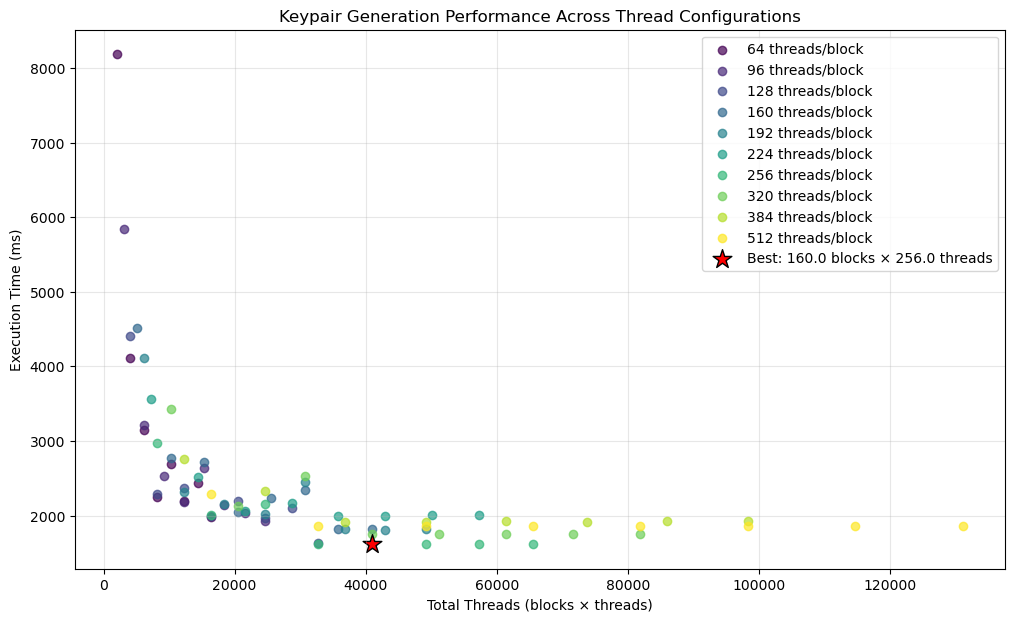
\includegraphics[width=\textwidth]{./fig/thread_time_cost.png}
      \centerline{block和thread配置下的性能对比}
    \end{column}
    \hfill
    \begin{column}{0.48\textwidth}
      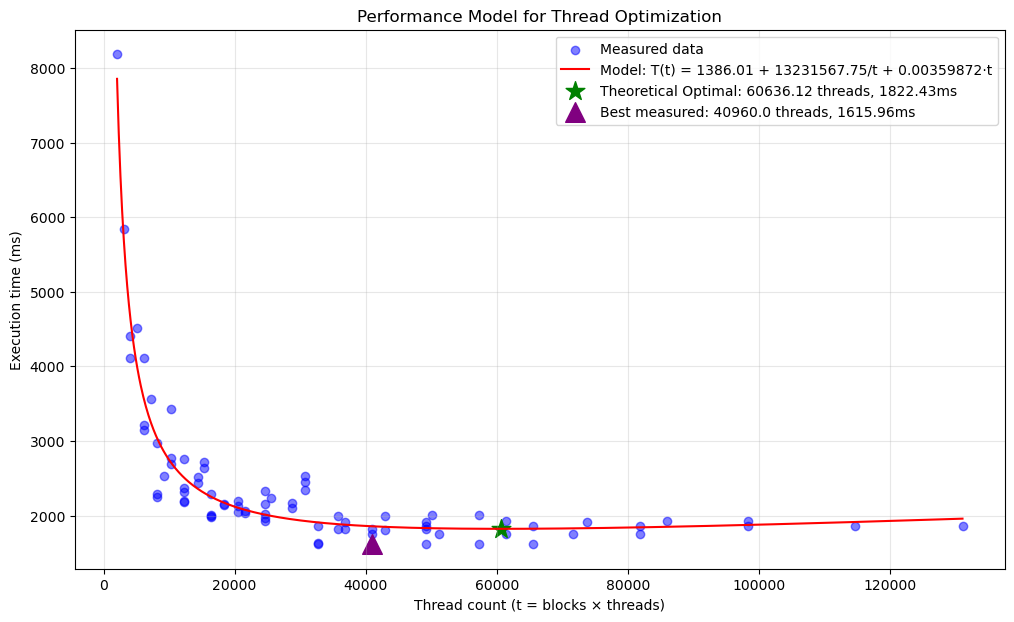
\includegraphics[width=\textwidth]{./fig/approach.png}
      \centerline{性能函数拟合曲线}
    \end{column}
  \end{columns}
  \vspace{0.5cm}
  \begin{itemize}
    \item 系统性测试了8种block数量(32-256)和10种thread数量(64-512)
    \item 通过函数拟合成功预测最优线程配置
    \item 签名处理时间从0.0605秒\cite{Wang2025}降至0.0493秒,提升17.4\%
  \end{itemize}
\end{frame}

\begin{frame}
  \frametitle{Thread与Block配置优化}
  \begin{center}
    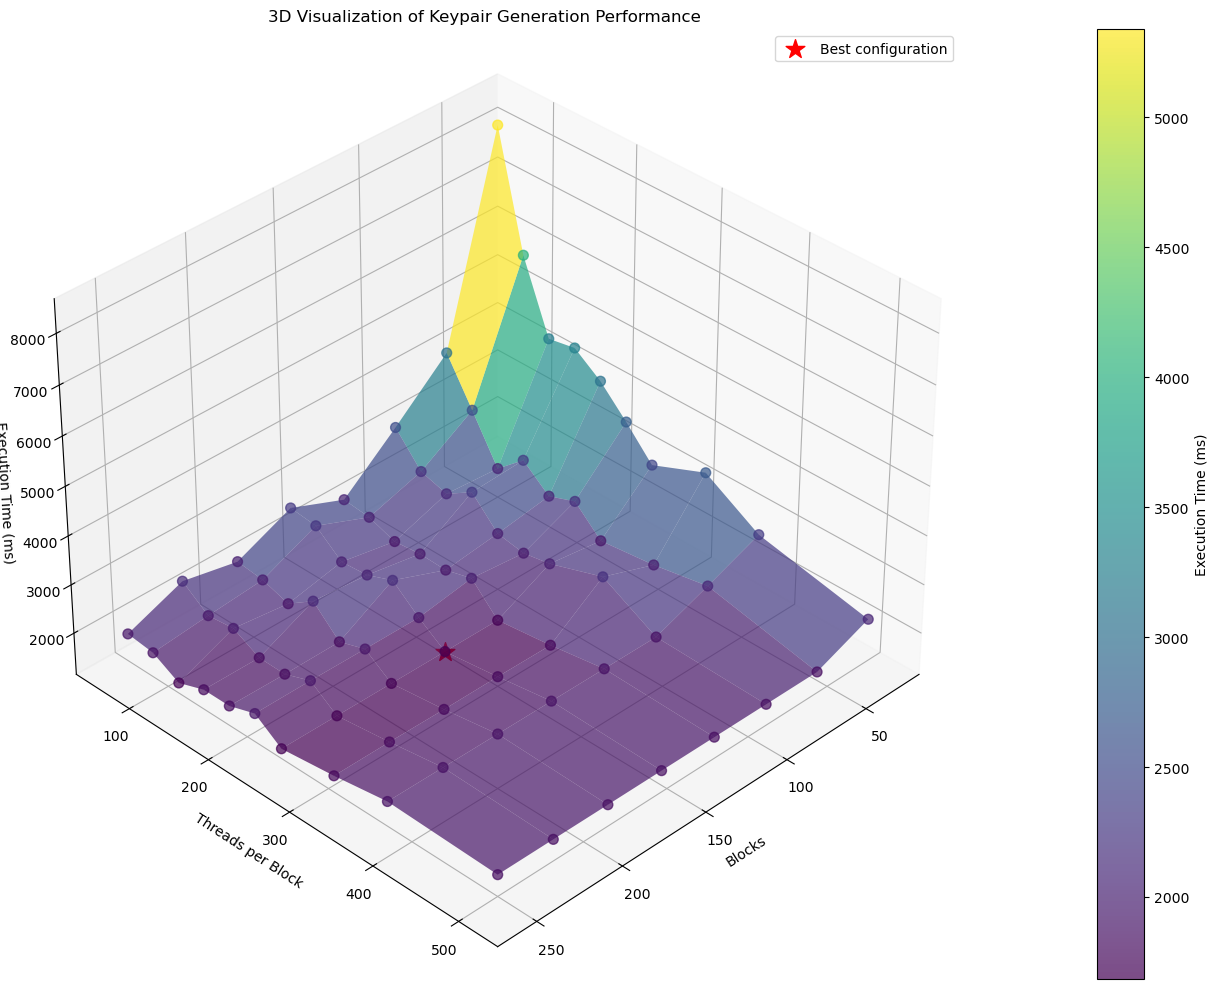
\includegraphics[width=0.7\textwidth]{./fig/block_thread_time.png}
  \end{center}
  \begin{itemize}
    \item 固定总并行度条件下,分析block和thread比例对性能的影响
    \item 每个block包含256个threads时达到最佳性能
    \item 找到明确的线程组织最优点,平衡线程管理开销与并行计算效率
  \end{itemize}
\end{frame}

\begin{frame}
  \frametitle{优化架构设计}
  \begin{center}
    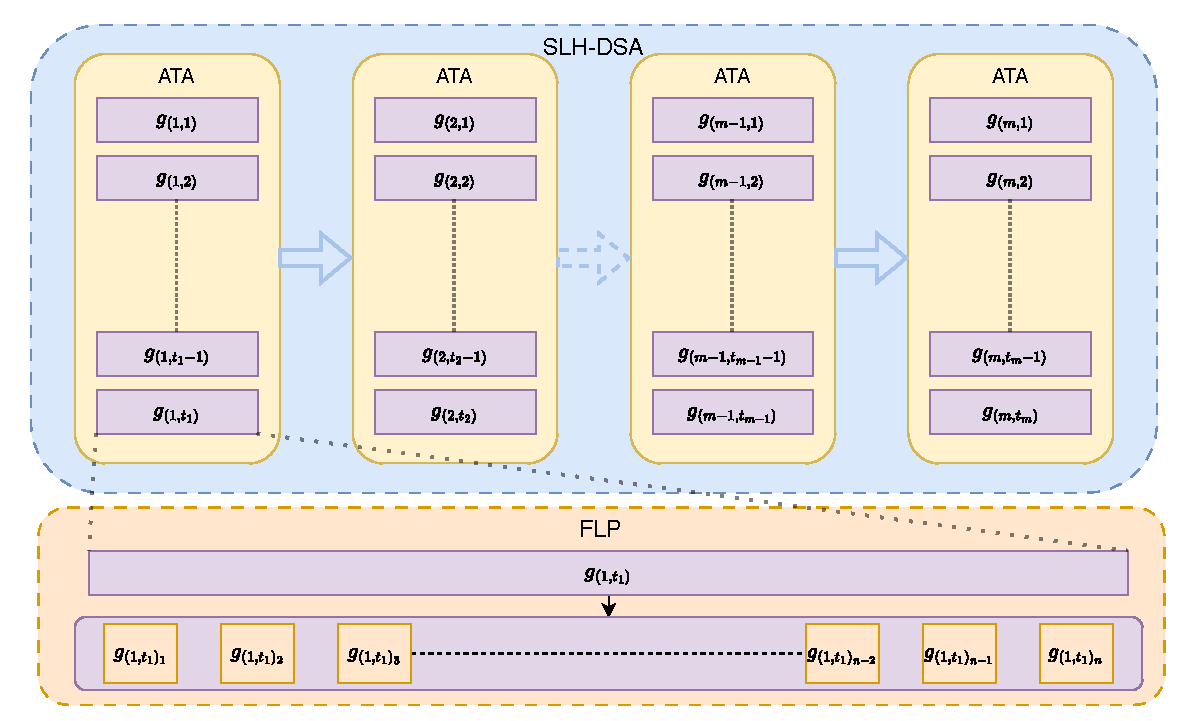
\includegraphics[width=0.7\textwidth]{./fig/optimize-overview.pdf}
  \end{center}
  \begin{itemize}
    \item 优化架构:
      \begin{itemize}
        \item 自适应线程分配(Adaptive Thread Allocation, ATA)
        \item 函数级并行(Function-Level Parallelism, FLP)
      \end{itemize}
    \item 作为论文核心图表,清晰传达优化方法论
  \end{itemize}
\end{frame}

\begin{frame}
  \frametitle{老师评语}
  \begin{alertblock}{论文的写作进展慢,还有就是写作语言很多没用书面正式语}
  参考trans短报论文,对写作进行优化
  \end{alertblock}
  \vfill
  \begin{block}{下周计划}
    \begin{enumerate}
        \item 开始论文实验章节书写
        \item 完善创新点2,函数级并行优化
    \end{enumerate}
  \end{block}
\end{frame}

\begin{frame}
  \frametitle{参考文献}
  \bibliographystyle{alpha}
  \bibliography{../../paper}
\end{frame}

\end{document}
